\section{Localizar mão de obra}

\par Uma das funcionalidades implementadas no desenvolvimento foi a busca por mão de obra. Esta busca permite que o usuário encontre profissionais que desempenhem a função específica procurada por ele. Para realizar esta busca, foi preciso escrever uma consulta que leva em conta três níveis de análise, sendo elas, a busca pelo profissional que desempenhe o trabalho dentro da rede de parceiros do usuário, dentro da empresa onde o ele trabalha e por último, dentro da cidade onde vive.  

\par Para escrever esta consulta foi utilizada a tecnologia \textit{Cypher}, que é uma linguagem específica para o banco Neo4j \cite{neo4j_team_manual}. O Código~\ref{list:consulta_busca} apresenta a \textit{query} utilizada para realizar esta busca.

\par A Figura~\ref{fig:busca_domestica_edilson} demonstra a página apresentada ao usuário após realizar esta busca por um determinado serviço. No exemplo, é apresentado o resultado ao se realizar a busca por um profissional que desempenhe o serviço de doméstica.

\begin{figure}[h!]
	\centerline{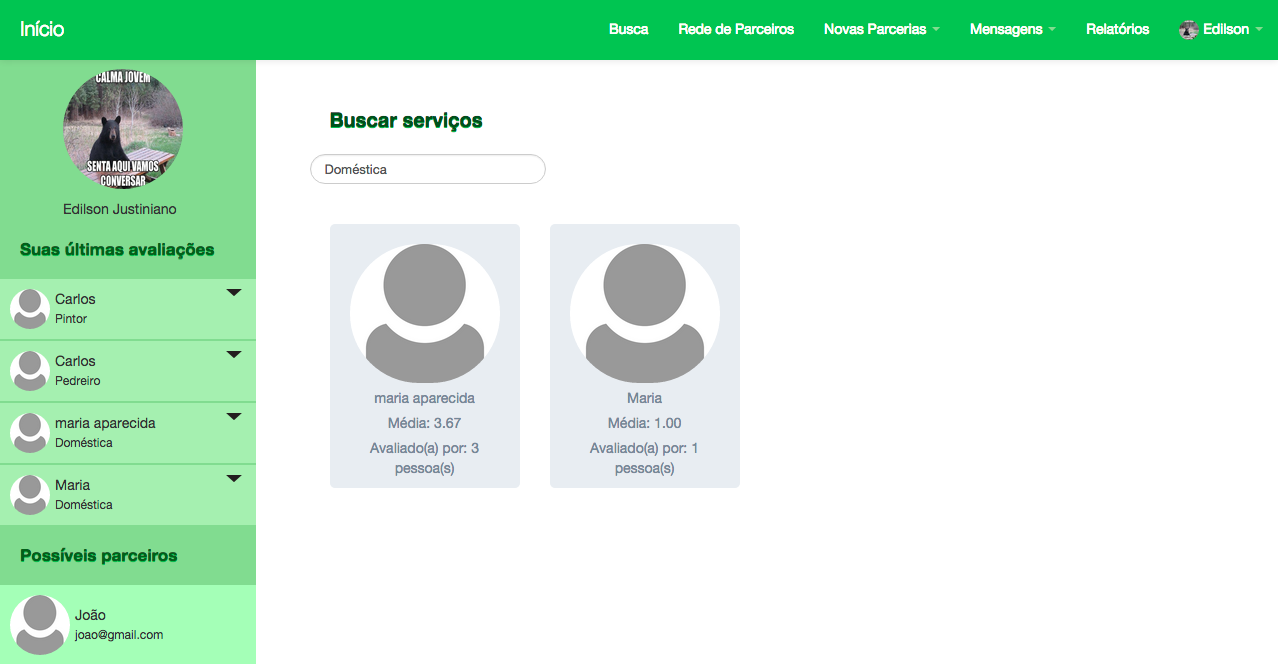
\includegraphics[scale=0.3]{./imagens/busca-domestica-edilson.png}}
	\caption[Página resultante da busca por doméstica.]
	{Página resultante da busca por doméstica. \textbf{Fonte:} Elaborado pelos autores.}
	\label{fig:busca_domestica_edilson}
\end{figure}

\par A ideia desta funcionalidade foi apresentar um possível prestador de serviços que já tenha sido avaliado por alguém em comum ao usuário solicitante, desta forma, há uma confiança maior em relação ao profissional que está sendo contratado. Portanto, essa busca irá apresentar diferentes prestadores de serviços, incluindo a média de cada um deles, a cada usuário solicitante.

%Seria uma conclusão e não uma discussão de resultado
%\par O uso de um banco de dados orientado a grafos como o Neo4j simplificou a forma de obter este resultado, uma vez que ao utilizar um banco relacional o mesmo resultado poderia ser obtido, porém o gasto em processamento e \textit{performance} seria extremamente maior. A API \textit{Cypher} facilitou a escrita de todas as consultas inclusive essa, por meio dela foi possível desenvolver consultas mais complexas como esta de forma mais rápida, agilizando o desenvolvimento da principal parte do trabalho.



